% !TeX root = ../../Skript.tex
\cohead{\Large\textbf{Bogenmaß}}
\fakesubsection{Bogenmaß}
\begin{minipage}{\textwidth}
	\adjustbox{valign=t}{\begin{minipage}{.5\textwidth}
		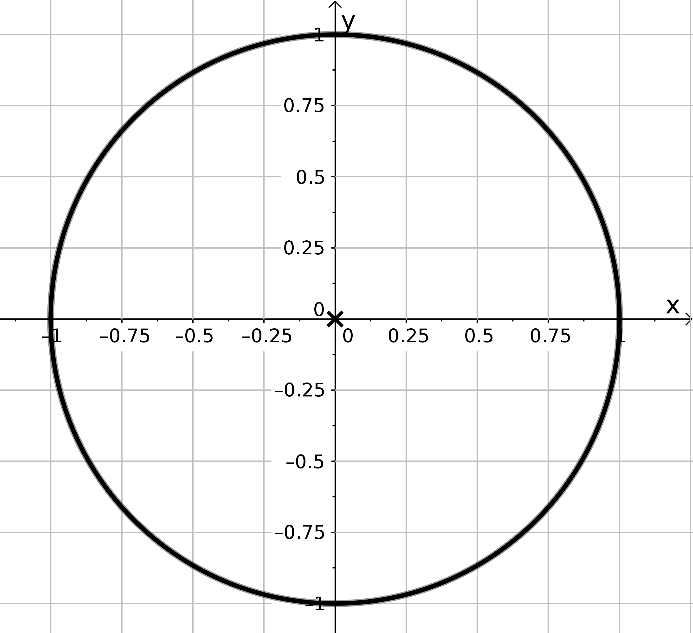
\includegraphics[width=\linewidth]{\trigonometrie/pics/Einheitskreis.png}
	\end{minipage}}%
	\adjustbox{valign=t, padding=3ex 0ex 0ex 0ex}{\begin{minipage}{.5\textwidth-3ex}\raggedright
		Um das Bogenmaß und später die Sinus- und Cosinusfunktion zu definieren, verwenden wir den Einheitskreis, also einen Kreis mit dem Radius 1.
		Im Bogenmaß wird der Winkel durch die Länge des entsprechenden Kreisbogens im Einheitskreis angegeben.

		\textcolor{loes}{\(\alpha\): Winkel im Gradmaß}

		\textcolor{loes}{\(b\): Länge des Kreisbogens und damit Winkel im Bogenmaß}
	\end{minipage}}%
\end{minipage}

\begin{tcolorbox}
	\textbf{Konvertieren von Bogenmaß in Gradmaß und umgekehrt:}

	\textcolor{loestc}{\[\frac{b}{2\pi}=\frac{\alpha}{360^\circ}\]
	}
\end{tcolorbox}


\begin{Exercise}[title={\raggedright\normalfont Bestimme jeweils das Grad- bzw. Bogenmaß.}, label=bogenmassA1]
	\begin{enumerate}[label=\alph*)]
		\item \(\alpha=30^\circ=\)
		\item \(\beta=270^\circ=\)
		\item \(\gamma=178^\circ=\)
		\item \(\delta=-15^\circ=\)
		\item \(\epsilon=0^\circ=\)
		\item \(\varphi=385^\circ=\)
		\item \(\eta=720^\circ=\)
		\item \(\theta=-95^\circ=\)
		\item \(\kappa=\frac{\pi}{2}=\)
		\item \(\lambda=\frac{7}{3}\pi=\)
		\item \(\mu=-\pi=\)
		\item \(\xi=5\pi=\)
		\item \(\rho=\frac{18\pi}{11}=\)
	\end{enumerate}
\end{Exercise}



%%%%%%%%%%%%%%%%%%%%%%%%%%%%%%%%%%%%%%%%%
\begin{Answer}[ref=bogenmassA1]
	\begin{enumerate}[label=\alph*)]
		\item \(\alpha=30^\circ=\frac{1}{6}\pi\)
		\item \(\beta=270^\circ=\frac{3}{2}\pi\)
		\item \(\gamma=178^\circ=\frac{89}{90}\pi\)
		\item \(\delta=-15^\circ=-\frac{1}{12}\pi\)
		\item \(\epsilon=0^\circ=0\)
		\item \(\varphi=385^\circ=\frac{77}{36}\pi\)
		\item \(\eta=720^\circ=4\pi\)
		\item \(\theta=-95^\circ=-\frac{19}{36}\pi\)
		\item \(\kappa=\frac{\pi}{2}=90^\circ\)
		\item \(\lambda=\frac{7}{3}\pi=420^\circ\)
		\item \(\mu=-\pi=-180^\circ\)
		\item \(\xi=5\pi=900^\circ\)
		\item \(\rho=\frac{18\pi}{11}=\frac{3240}{11}^\circ\approx294,54^\circ\)
	\end{enumerate}
\end{Answer}